\documentclass[final]{beamer}
%% Possible paper sizes: a0, a0b, a1, a2, a3, a4.
%% Possible orientations: portrait, landscape
%% Font sizes can be changed using the scale option.
\usepackage[size=a0,orientation=portrait]{beamerposter}

\usepackage{euler}
\usetheme{gemini}
% \usecolortheme{seagull}

% ====================
% Packages
% ====================

\usepackage[utf8]{inputenc}
\usepackage{graphicx}
\usepackage{booktabs}
\usepackage{tikz}
\usepackage{pgfplots}

% ====================
% Lengths
% ====================

% If you have N columns, choose \sepwidth and \colwidth such that
% (N+1)*\sepwidth + N*\colwidth = \paperwidth
\newlength{\sepwidth}
\newlength{\colwidth}
\setlength{\sepwidth}{0.005\paperwidth}
\setlength{\colwidth}{0.48\paperwidth}

\newlength{\vboxsep}
\setlength{\vboxsep}{-.6\baselineskip}
\newlength{\mboxpreadjust}
\setlength{\mboxpreadjust}{-.4\baselineskip}

\newcommand{\separatorcolumn}{\begin{column}{\sepwidth}\end{column}}




%!TEX root = xprag-poster.tex

%% extra 

% colors

	\definecolor{maintheme}{cmyk}{.71, .51, 0, 0}
	\definecolor{highlight}{cmyk}{.05, .8, .05, 0}
	\definecolor{lowlight}{cmyk}{.64, .5, 0, .09}
	\definecolor{sechighlight}{cmyk}{0, .31, 100, .10}

	% \setbeamercolor{alerted text}{fg=orange}
	\setbeamercolor{background canvas}{bg=white}
	% \setbeamercolor{block body alerted}{bg=normal text.bg!90!black}
	\setbeamercolor{block body}{bg=normal text.bg!90!black}
	% \setbeamercolor{block body example}{bg=normal text.bg!90!black}
	% \setbeamercolor{block title alerted}{use={normal text,alerted text},fg=alerted text.fg!75!normal text.fg,bg=normal text.bg!75!black}
	% \setbeamercolor{block title}{bg=blue}
	% \setbeamercolor{block title example}{use={normal text,example text},fg=example text.fg!75!normal text.fg,bg=normal text.bg!75!black}
	% \setbeamercolor{fine separation line}{}
	% \setbeamercolor{frametitle}{fg=brown}
	% \setbeamercolor{item projected}{fg=black}
	\setbeamercolor{normal text}{fg=black}
	\setbeamercolor{caption name}{fg=black}
	% \setbeamercolor{separation line}{}
	\setbeamercolor{structure}{fg=maintheme}
	\setbeamercolor{title}{fg=maintheme, bg=lowlight}
	% \setbeamercolor{titlelike}{fg=maintheme}

	\definecolor{modal}{cmyk}{0, .31, 100, .0}
	\definecolor{cond}{cmyk}{.8, 0, .3, .3}
	\definecolor{neg}{cmyk}{.63, .23, 0, .0}
	\definecolor{question}{cmyk}{1, .36, 0, .30}

	\definecolor{red}{cmyk}{0,1,.5,0}

% boxes
	\usepackage{tcolorbox}
	\tcbuselibrary{skins}

	\newtcbox{\predhighlight}[1][lowlight]{on line,
	arc=3pt,colback=#1!10!white,colframe=#1!50!black,
	before upper={\rule[-3pt]{0pt}{10pt}},boxrule=1pt,
	boxsep=0pt,left=2pt,right=2pt,top=1pt,bottom=.5pt}

	\newtcbox{\ophighlight}[1][highlight]{on line,
	arc=3pt,colback=#1!10!white,colframe=#1!50!black,
	before upper={\rule[-3pt]{0pt}{10pt}},boxrule=1pt,
	boxsep=0pt,left=2pt,right=2pt,top=1pt,bottom=.5pt}

	\newtcolorbox{normalbox}[1]{colback=white,colframe=maintheme,fonttitle=\bfseries\Raleway\large,
	title={#1}}

	% \tcbset{colback=red!5!white,fonttitle=\bfseries}
	% \newtcolorbox{upshotbox}[1]{enhanced, squeezed title={#1}, frame style={left color=highlight, right color=lowlight!75!black}, leftrule=3mm, fonttitle=\bfseries\Raleway\Large, colback=highlight!5!white
	% }

	\newtcolorbox{upshotbox}[1]{
		colframe=highlight,
		colback=highlight!5!white,
		% colframe=maintheme,
		% colback=white,
		% coltitle=maintheme,
		adjusted title=center,halign title=center,
		title={#1},
		% frame style={left color=highlight, right color=lowlight!75!black},
		leftrule=3mm,
		fonttitle=\bfseries\Raleway\Large,
		%
		% detach title, before upper={\centering\tcbtitle\par}
	}

	\newtcolorbox{modelbox}[1]{
		% colback=lowlight!5!white,
		% colframe=lowlight,
		% coltitle=lowlight,
		colback=white,
		colframe=maintheme,
		coltitle=maintheme,
		text width=.95\linewidth,
		title={#1},
		fonttitle=\bfseries\footnotesize,
		detach title, before upper={\tcbtitle\par},
	}

	\newtcolorbox{theorybox}[1]{
		% colback=lowlight!5!white,
		% coltitle=lowlight,
		% colframe=lowlight,
		colback=white,
		colframe=maintheme,
		coltitle=maintheme,
		text width=.85\linewidth,
		title={#1},
		fonttitle=\bfseries\small,
		detach title, before upper={\tcbtitle\par},
	}

	\newtcolorbox{questionbox}[1]{
		colback=question!5!white,
		colframe=question,
		coltitle=question,
		% text width=.78\linewidth,
		title={#1},
		fonttitle=\bfseries,
		detach title, before upper={\tcbtitle},
	}

	\newtcolorbox{negbox}[1]{
		colback=neg!5!white,
		colframe=neg,
		coltitle=neg,
		% text width=.78\linewidth,
		title={#1},
		fonttitle=\bfseries,
		detach title, before upper={\tcbtitle},
	}

	\newtcolorbox{modalbox}[1]{
		colback=modal!5!white,
		colframe=modal,
		coltitle=modal,
		% text width=.78\linewidth,
		title={#1},
		fonttitle=\bfseries,
		detach title, before upper={\tcbtitle},
	}

	\newtcolorbox{condbox}[1]{
		colback=cond!5!white,
		colframe=cond,
		coltitle=cond,
		% text width=.78\linewidth,
		title={#1},
		fonttitle=\bfseries,
		detach title, before upper={\tcbtitle},
	}

	\newtcbox{\qhl}[1][lowlight]{on line,
	arc=3pt,colback=question!5!white,colframe=question,
	coltitle=question,
	before upper={\rule[-3pt]{0pt}{10pt}},boxrule=1pt,
	boxsep=0pt,left=2pt,right=2pt,top=1pt,bottom=.5pt}

	\newtcbox{\nhl}[1][lowlight]{on line,
	arc=3pt,colback=neg!5!white,colframe=neg,
	coltitle=neg,
	before upper={\rule[-3pt]{0pt}{10pt}},boxrule=1pt,
	boxsep=0pt,left=2pt,right=2pt,top=1pt,bottom=.5pt}

	\newtcbox{\mhl}[1][lowlight]{on line,
	arc=3pt,colback=modal!5!white,colframe=modal,
	coltitle=modal,
	before upper={\rule[-3pt]{0pt}{10pt}},boxrule=1pt,
	boxsep=0pt,left=2pt,right=2pt,top=1pt,bottom=.5pt}

	\newtcbox{\chl}[1][lowlight]{on line,
	arc=3pt,colback=cond!5!white,colframe=cond,
	coltitle=cond,
	before upper={\rule[-3pt]{0pt}{10pt}},boxrule=1pt,
	boxsep=0pt,left=2pt,right=2pt,top=1pt,bottom=.5pt}

% beamer elements
	% \useinnertheme{rounded}
	\setbeamertemplate{item}{\scriptsize$\blacktriangleright$}

% misc formatting
	\usepackage{linguex}
	\usepackage{booktabs}
	\usepackage[round]{natbib}
	\usepackage{multirow}
	\usepackage{rotating}

% drawing

	\usepackage{tikz}

% symbols 
	\usepackage{pifont}% http://ctan.org/pkg/pifont
	\newcommand{\cmark}{\ding{51}}%
	\newcommand{\xmark}{\ding{55}}%




%% Reference Sources
% \addbibresource{refs.bib}

\title{Projection variability of clausal complements across different operators}

\author{Lisa Hofmann\inst{1} \and Marie-Catherine de Marneffe\inst{2} \and Judith Tonhauser\inst{1}}

\institute[shortinst]{\inst{1} University of Stuttgart \samelineand \inst{2} UC Lovain}

\date{\today}

\begin{document}
	
\begin{frame}[t]

	\vspace{-2cm}
	\begin{columns}[t]
		\separatorcolumn
		
		\begin{column}{.74\colwidth}
			\begin{upshotbox}{Does the projection of content differ across entailment-canceling environments?}

				\begin{itemize}
					\item[\color{highlight}{$\blacktriangleright$}] \textbf{Yes!} Projection differs by entailment-cancelling \ophighlight{operator}
						
					\item[\color{highlight}{$\blacktriangleright$}] By-operator effects differ by predicate (\textbf{\ophighlight{operator}/\predhighlight{predicate} interaction})
					
					\item[\color{highlight}{$\blacktriangleright$}] Current theories of \cchighlight{projective content} do not predict our results
				\end{itemize}
				
			\end{upshotbox}
			\vspace{\vboxsep}
			\begin{normalbox}{Projection of clausal complements}
				Do you infer that Rachel is committed to the truth of the \textit{content of the complement} (CC), that \cchighlight{Julian dances salsa}?
				
				\vspace{-.3\baselineskip}
				\ex. \a. Rachel: \emph{\lq Does Cole \predhighlight{know} that \cchighlight{Julian dances salsa}?\rq}\\
					\cmark\ \  Yes, CC projects out of the question
					\b. Rachel: \emph{\lq Does Cole \predhighlight{think} that \cchighlight{Julian dances salsa}?\rq}\\
					\xmark\ \ No, CC does not project
					\z.
				\z.
				
				\vspace{-.5\baselineskip}
				\resizebox{\linewidth}{!}{
					\begin{minipage}{1.7\linewidth}
						\citet{frege_uber_1892,strawson_referring_1950,kiparsky_fact_1970,karttunen_observations_1971,karttunen_conventional_1979}, and many more

					\end{minipage}
				}
			\end{normalbox}

			\vspace{\vboxsep}
			\begin{normalbox}{Entailment-cancelling operators}
				\textbf{Family-of-sentences test:}\newline No mention of differences in projection between different \ophighlight{operators}
				
				\vspace{-.5\baselineskip}
				\ex. \a. Polar question:\\
					\textit{\ophighlight{Does} Cole \predhighlight{know} that \cchighlight{Julian dances salsa}?}
					\b. Negation:\\
					\textit{Cole \ophighlight{doesn't} \predhighlight{know} that \cchighlight{Julian dances salsa}.}
					\b. Epistemic modal:\\
					\textit{\ophighlight{Perhaps} Cole \predhighlight{knows} that \cchighlight{Julian dances salsa}.}
					\b. Conditional antecedents:\\
					\textit{\ophighlight{If} Cole \predhighlight{knows} that \cchighlight{Julian dances salsa}, Logan will be joyful.}
					\z.
				\z.

				\vspace{-.5\baselineskip}
				\resizebox{\linewidth}{!}{
					\begin{minipage}{1.7\linewidth}
						(e.g. \citealt{chierchia_meaning_1990,coppock_invitation_2020})

					\end{minipage}
				}

			\end{normalbox}
			
			\vspace{\vboxsep}
			\begin{normalbox}{Hints at by-operator variation}
				\textbf{Factive vs. semi-factive predicates} (\citealt{karttunen_observations_1971})
				\vspace{-.2\baselineskip}
				\begin{itemize}
					\item Factives (\textit{be annoyed, regret, \dots}): CC projects across all four operators
					\item Semi-factives (\textit{discover, realize, see, notice, \dots}):\newline CC projects across negation, but not always for the other operators
				\end{itemize}

				\textbf{Experiment with English projective contents} (\citealt{smith_relationship_2014})
				\vspace{-.2\baselineskip}
				\begin{itemize}
					\item Projective content of epithets (e.g. \textit{idiot}) and the CC of \textit{know}:\\ more projective under negation than conditionals
					\item Opposite pattern for appositive relative clauses and \textit{win}
				\end{itemize}

				\textbf{Experiment with German clause-embedding predicates}\\ (\citealt{sieker_projective_2022})
				\vspace{-.2\baselineskip}
				\begin{itemize}
					\item Higher projection ratings w/ negation than other three operators
					\item No by-predicate variation, no evidence for factive/semi-factive distinction
				\end{itemize}

				\begin{figure}[h]
					\vspace{-.2\baselineskip}
					\centering
					\includegraphics[width=.7\linewidth]{sieker-solstad.png}
					\vspace{-.4\baselineskip}
					\caption{\citealt{sieker_projective_2022}, p. 286: Projection-ratings by embedding operator, for purported factive and semi-factive predicates}
					% \label{fig:figure1}
				\end{figure}
				\vspace{-.8\baselineskip}
			\end{normalbox}

			\vspace{\vboxsep}
			\begin{normalbox}{Certain-that task for projection inferences}

				\begin{figure}[h]
					\centering
					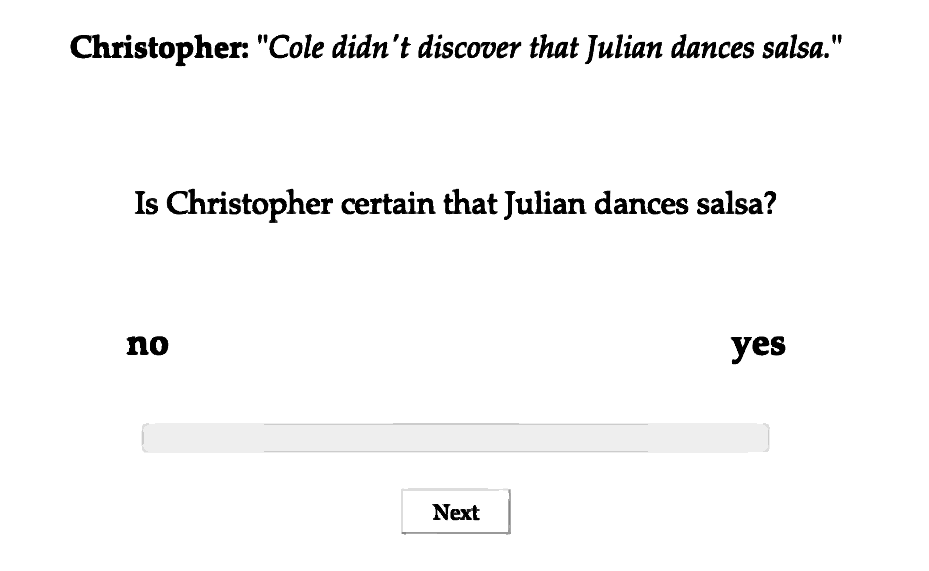
\includegraphics[width=.6\linewidth]{task-1n-proj.eps}
					% \caption{Caption here}
					\label{fig:task}
				\end{figure}

				\resizebox{\linewidth}{!}{
					\begin{minipage}{1.7\linewidth}
						\citet{tonhauser_prosodic_2016,djarv_prosodic_2017,tonhauser_how_2018,de_marneffe_commitmentbank_2019,mahler_social_2020,degen_are_2022,sieker_projective_2022}

					\end{minipage}
				}
				
			\end{normalbox}

			\vspace{\vboxsep}
			\begin{normalbox}{Variation among clause-embedding predicates}
				20 \predhighlight{predicates} that have shown projection variability in PQs\newline (\citealt{degen_are_2022})

				\begin{figure}[h]
					\centering
					\includegraphics[width=.95\linewidth]{degen-tonhauser.png}
					\caption{\citealt{degen_are_2022}, p. 562: Mean certainty ratings by predicate}
					\label{fig:task}
				\end{figure}
				\vspace{-.8\baselineskip}
			\end{normalbox}

			\vspace{\vboxsep}
			\begin{normalbox}{Materials}
				To assess the effect of \ophighlight{operator} and \predhighlight{predicate} on \cchighlight{\textbf{projection}}:
				\vspace{.2\baselineskip}

					\textbf{4 experiments} (roughly $750$ participants each)
					\vspace{-.3\baselineskip}
					\begin{itemize}
						\item One per \ophighlight{operator}: polar questions, negation, modal \textit{perhaps}, conditional
					\end{itemize}

					\vspace{-.2\baselineskip}
					Participants saw:
					\vspace{-.3\baselineskip}
					\begin{itemize}
						\item \textbf{20 clause embedding \predhighlight{predicates}}

						\begin{itemize}
							\item  Crossed with 20 CCs ($20 \times 20 = 400$ combinations)
						\end{itemize}

						\item (6 controls for exclusion)

					\end{itemize}
				\vspace{-.2\baselineskip}
				{\small (Experiments also used different at-issueness measures in separate block, not analyzed here)}

			\end{normalbox}
			
		\end{column}

		\separatorcolumn
		
		\begin{column}{1.25\colwidth}
			\begin{normalbox}{Main effect of embedding operator \& By-predicate variation in the effect of operator}
				% \vspace{-\baselineskip}
				\hspace{-.2cm}\begin{tabular}{p{.70\linewidth} p{.3\linewidth}}
					\textcolor{highlight}{\large \Raleway By-operator variation aggregating across predicates (Figure 3)}
					\begin{itemize}
						\item Conditional > Question > Negation, Modal
							\vspace{\mboxpreadjust}
							\begin{modelbox}{Model \#1: Linear mixed effect regression}
								\footnotesize
								response: \textbf{certainty ratings}; fixed effect: \ophighlight{\textbf{operator}} (base level: Question);
								random intercepts: participants, items; \newline
								MLEs: question (intercept) $0.51$, conditional $+0.05$, modal $-0.04$, negation $-0.03$; with all $p < 0.001$
							\end{modelbox}

						\item But small differences, as in Sieker \& Solstad’s (2022) study
						\item Sieker \& Solstad’s results for German: Negation > Question, Conditional, Modal

					\end{itemize}

				\textcolor{highlight}{\large \Raleway Effect of operator differs by predicate (Figure 4), e.g.}
				\begin{itemize}
					\item CC of \predhighlight{be annoyed}: Negation, Conditional > Question, Modal
						\vspace{\mboxpreadjust}
						\begin{modelbox}{Model \#2: Linear mixed effect regression}
							\footnotesize
							response: \textbf{certainty ratings}; fixed effects: \ophighlight{operator}, \predhighlight{predicate}, and interaction (base level: \textbf{be annoyed} / negation); random intercepts: participant; \newline
							MLEs: negation (intercept) $0.87$, conditional $-0.12$, modal $-0.16$; with $p < 0.001$; question $+0.02$ (n.s.)
						\end{modelbox}

					\item CC of \predhighlight{know}: Question > Negation, Conditional > Modal
						\vspace{\mboxpreadjust}
						\begin{modelbox}{Model \#3: Linear mixed effect regression}
							\footnotesize
							response: \textbf{certainty ratings}; fixed effects: \ophighlight{operator}, \predhighlight{predicate}, and interaction (base level: \textbf{know} / negation); random intercepts: participant; \newline
							MLEs: negation (intercept) $0.79$, modal $-0.14$, question $+0.08$; with $p < 0.001$; , conditional $+/- 0$, (n.s.)
						\end{modelbox}

					\item CC of \predhighlight{discover}: Modal > Negation > Conditional, Question
						\vspace{\mboxpreadjust}
						\begin{modelbox}{Model \#4: Linear mixed effect regression}
							\footnotesize
							response: \textbf{certainty ratings}; fixed effects: \ophighlight{operator}, \predhighlight{predicate}, and interaction (base level: \textbf{discover} / negation); random intercepts: participant; \newline
							MLEs: negation (intercept) $0.68$, conditional $+0.11$, modal $-0.06$, question $+0.10$; with $p < 0.001$
						\end{modelbox}

				\end{itemize}

					&

					\vspace{-1.25\baselineskip}
					\begin{figure}[h]
						% \hspace{-1cm}
						\centering
						\includegraphics[width=.9\linewidth]{projective-op.pdf}
						\vspace{-\baselineskip}
						\caption{Mean certainty ratings by operator}
						\label{fig:figure2}
					\end{figure}
				\end{tabular}
				\vspace{-\baselineskip}
				\begin{figure}[h]
					\centering
					\includegraphics[width=\linewidth]{projective-pred-op.pdf}
					\vspace{-2\baselineskip}
					\caption{Mean certainty ratings by predicate, grouped by operator}
					\label{fig:figure3}
				\end{figure}
				\vspace{-.8\baselineskip}
			\end{normalbox}
			
			\vspace{\vboxsep}	
			\begin{normalbox}{Discussion --- By predicate variation in the effect of operator}
				\begin{itemize}
					\item Concurs with \citet{smith_relationship_2014}, who found content/operator interactions for English projective contents
					\item Differs from \citet{sieker_projective_2022}, who found no predicate/operator interaction for CCs of German clause-embedding predicates
				\end{itemize}
				
				\textbf{No evidence for factive vs. semi-factive distinction (\citealt{karttunen_observations_1971})}
				\begin{itemize}
					\item CC of purported factive \textit{be annoyed} does not invariably project across operators
					\item CC of purported semi-factives (\textit{discover, see}) do not project more across negation than other operators
				\end{itemize}

				\textbf{Provides support (from negation, modals, conditionals) for Degen \& Tonhauser’s (2022) result:}
				\begin{itemize}
					\item Projection does not categorically differentiate between (semi-)factive/-factive predicates 
				\end{itemize}
				
			\end{normalbox}

			\vspace{\vboxsep}
			\begin{normalbox}{Do existing theories of projection predict our results?}
				\textbf{Dynamic accounts of projection: Lexical factivity \& dynamic operators} \hfill (\citealt{heim_projection_1983,van_der_sandt_presupposition_1992})

				Distinguish factive and non-factive predicates:
				\begin{itemize}
					\item factive predicates (\textit{be annoyed, regret, \dots}): CC conventionally required to be contextually entailed in common ground

					\item non-factive predicates (\textit{believe, say, …}): no such requirement

				\end{itemize}
				
				Factive content projects globally, unless not admitted by common ground

				\textbf{Entailments \& discourse structure} \hfill (\citealt{abrusan_predicting_2011,simons_best_2017})

				\textbf{Contextual entailments \& Epistemic preconditions} \hfill (\citealt{schlenker_triggering_2021})

			\end{normalbox}

			\vspace{\vboxsep}
			\begin{upshotbox}{Theoretical implications}
				\begin{itemize}
					\item Previous work: projection analyses need to consider the effect of \textbf{lexical meaning} (e.g. \citealt{kiparsky_fact_1970,karttunen_observations_1971}, et. seq.), \textbf{world knowledge} (\citealt{de_marneffe_did_2012,degen_prior_2021}), and \textbf{discourse structure} (e.g. \citealt{simons_best_2017,tonhauser_how_2018})
					
					\item Add to that the effect of various \ophighlight{entailment-cancelling operators}
					
					\item An analysis of projection should be able to address \ophighlight{operator} / \predhighlight{predicate} interaction effects. None of the extant projection analyses capture our data.

				\end{itemize}
			\end{upshotbox}

			\vspace{\vboxsep}
			\begin{normalbox}{References}
				\tiny
				
				\textbf{Márta Abrusán}. Predicting the presuppositions of soft triggers. \textit{Linguistics and philosophy}, 34:491–535, 2011. \quad \textbullet \quad
				%
				\textbf{Gennaro Chierchia and Sally McConnell-Ginet.} \textit{Meaning and grammar: An introduction to semantics.} 1990. \quad \textbullet \quad
				%
				\textbf{Elizabeth Coppock and Lucas Champollion.} \textit{Invitation to formal semantics.} online publication, in progress, 2020. \quad \textbullet \quad
				%
				\textbf{Marie de Marneffe, Mandy Simons, and Judith Tonhauser.} The CommitmentBank: Investigating projection in naturally occurring discourse. \textit{Sinn und Bedeutung}, 23:107–124, 2019. \quad \textbullet \quad
				%
				\textbf{Marie-Catherine de Marneffe, Christopher D. Manning, and Christopher Potts.} Did It Happen? The Pragmatic Complexity of Veridicality Assessment. \textit{Computational Linguistics}, 38(2):301–333, February 2012. \quad \textbullet \quad
				%
				\textbf{Judith Degen and Judith Tonhauser.} Prior beliefs modulate projection. \textit{Open Mind}, 5:59–70, 2021. \quad \textbullet \quad
				%
				\textbf{Judith Degen and Judith Tonhauser.} Are there factive predicates? An empirical investigation. \textit{Language}, 98(3):552–591, 2022. \quad \textbullet \quad
				%
				\textbf{Kajsa Djärv and Hezekiah Akiva Bacovcin.} Prosodic effects on factive presupposition projection. \textit{Semantics and Linguistic Theory}, 27:116–133, 2017. \quad \textbullet \quad
				%
				\textbf{Gottlob Frege.} Über Sinn und Bedeutung. \textit{Zeitschrift für Philosophie und philosophische Kritik}, pages 25–50, 1892. \quad \textbullet \quad
				%
				\textbf{Irene Heim.} On the projection problem for presuppositions. \textit{Formal semantics–the essential readings}, pages 249–260, 1983. \quad \textbullet \quad
				%
				\textbf{Lauri Karttunen.} Some observations on factivity. \textit{Research on Language \& Social Interaction}, 4(1):55–69, 1971. \quad \textbullet \quad
				%
				\textbf{Lauri Karttunen and Stanley Peters.} Conventional implicature. In Choon-Kyu Oh and David A. Dinneen, editors, \textit{Presuppositions, Syntax and Semantics} Vol.11, pages 1–56. New York: Academic Press, 1979. \quad \textbullet \quad
				%
				\textbf{Paul Kiparsky and Carol Kiparsky.} Fact. In Manfred Bierwisch and Karl Erich Heidolph, editors, \textit{Progress in Linguistics}, pages 143–173. The Hague: Mouton, 1970. \quad \textbullet \quad
				%
				\textbf{Taylor Mahler.} The social component of projection behavior of clausal complements. \textit{Linguistic Society of America}, 5:777–791, 2020. \quad \textbullet \quad
				%
				\textbf{Philippe Schlenker.} Triggering presuppositions. \textit{Glossa: a journal of general linguistics}, 6(1), 2021. \quad \textbullet \quad
				%
				\textbf{Judith Sieker and Torgrim Solstad.} Projective variability of (semi) factive verbs in family of sentence contexts: A rating study. \textit{In Proceedings of the 23rd Amsterdam Colloquium}, 2022. \quad \textbullet \quad
				%
				\textbf{Mandy Simons, David Beaver, Craige Roberts, and Judith Tonhauser.} The best question: Explaining the projection behavior of factives. \textit{Discourse processes}, 54(3):187–206, 2017. \quad \textbullet \quad
				%
				\textbf{E. Allyn Smith and Kathleen Currie Hall.} The relationship between projection and embedding environment. \textit{In Proceedings of the 48th Meeting of the Chicago Linguistics Society}. 2014. \quad \textbullet \quad
				%
				\textbf{Peter F. Strawson.} On referring. \textit{Mind}, 59(235):320–344, 1950. \quad \textbullet \quad
				%
				\textbf{Judith Tonhauser.} Prosodic cues to presupposition projection. In \textit{Semantics and Linguistic Theory}, volume 26, pages 934–960, 2016. \quad \textbullet \quad
				%
				\textbf{Judith Tonhauser, David I. Beaver, and Judith Degen.} How projective is projective content? Gradience in projectivity and at-issueness. \textit{Journal of Semantics}, 35(3):495–542, 2018. \quad \textbullet \quad
				%
				\textbf{Rob A. van der Sandt.} Presupposition projection as anaphora resolution. \textit{Journal of semantics}, 9(4):333–377, 1992.

			\end{normalbox}

			\begin{normalbox}{References (not visible later)}
				\bibliographystyle{plainnat}
				\bibliography{projection}
			\end{normalbox}

		\end{column}
		\separatorcolumn
	\end{columns}



\end{frame}
\end{document}